\chapter{Generaliserade integraler}
Vilka funktioner går att derivera?
Kontinuerliga?
Självklart, men behöver inte ens kontinuitet.
Till exempel:\\
% infoga bild 1
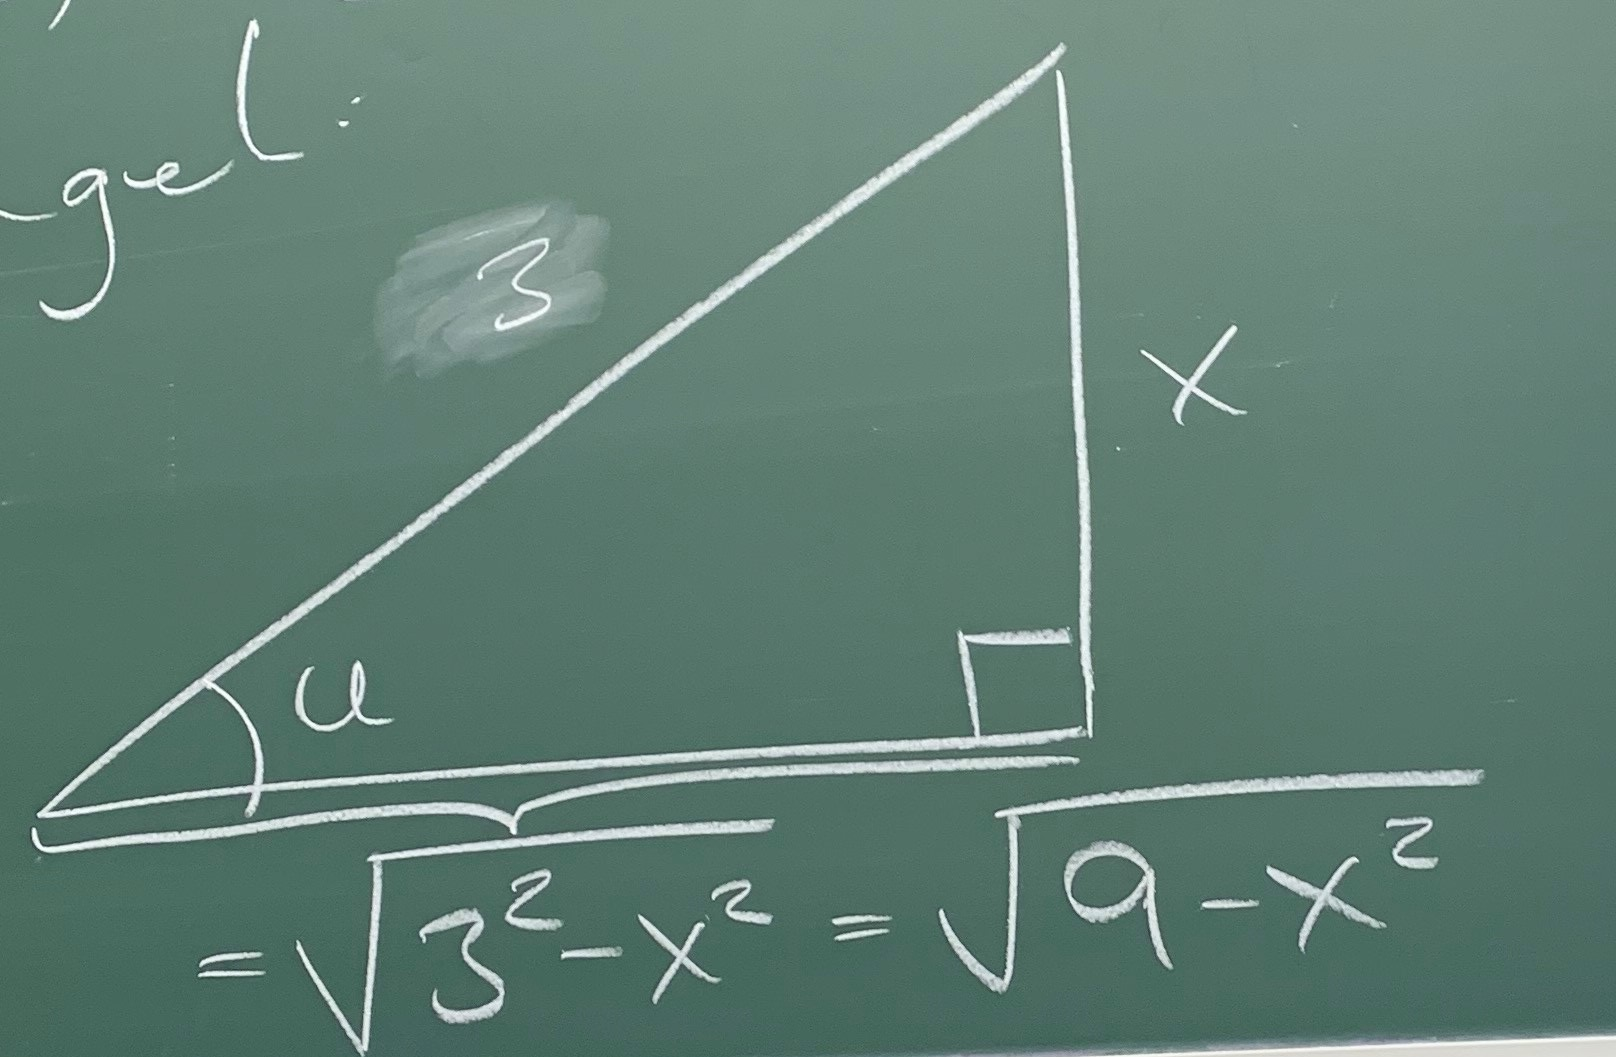
\includegraphics[scale=0.1]{lessons/lesson18/imgs/img01.jpg}\\

Värre kan det dock bli om antingen:
\begin{itemize}
    \item $f$ är obegränsad i någon punkt $x\in[a,b]$ 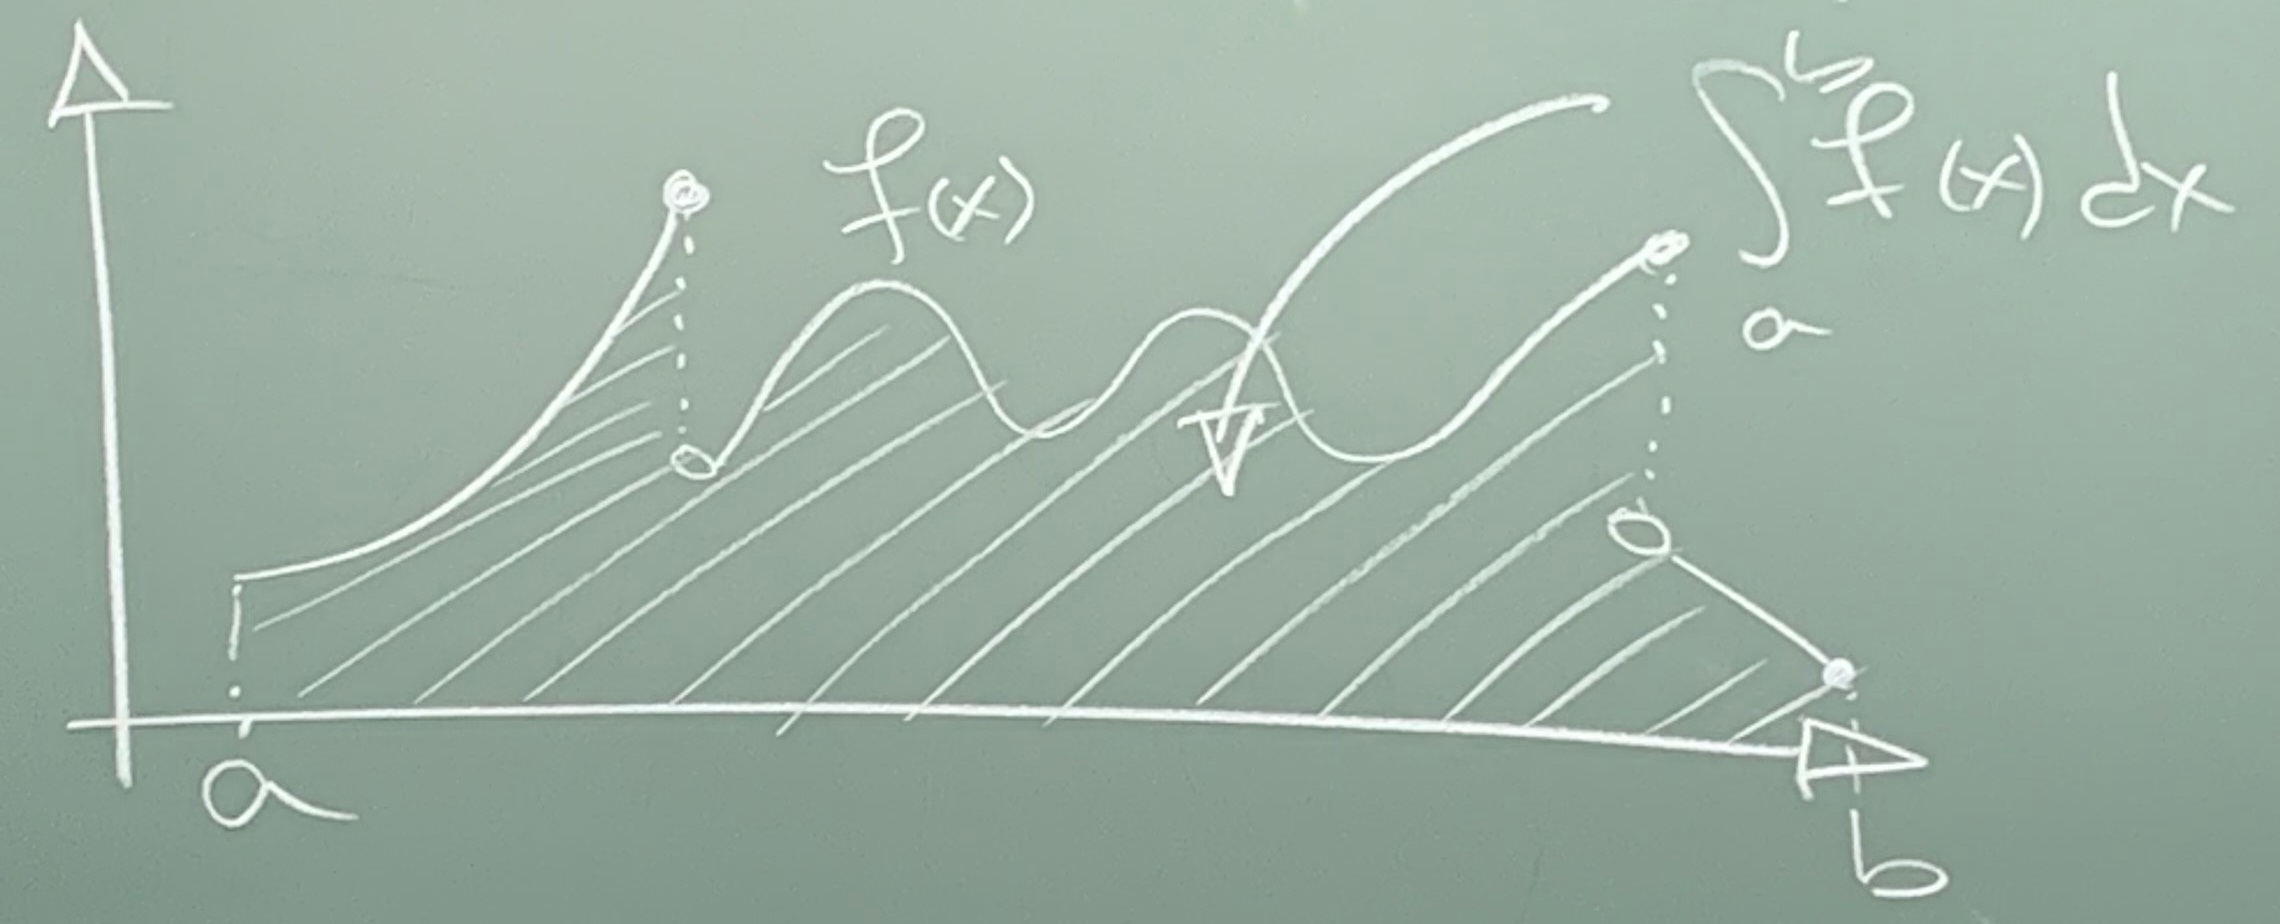
\includegraphics[scale=0.05]{lessons/lesson18/imgs/img02.jpg}%infoga bild 2 här
    \item $"a=-\infty"$ eller $b=\infty$ 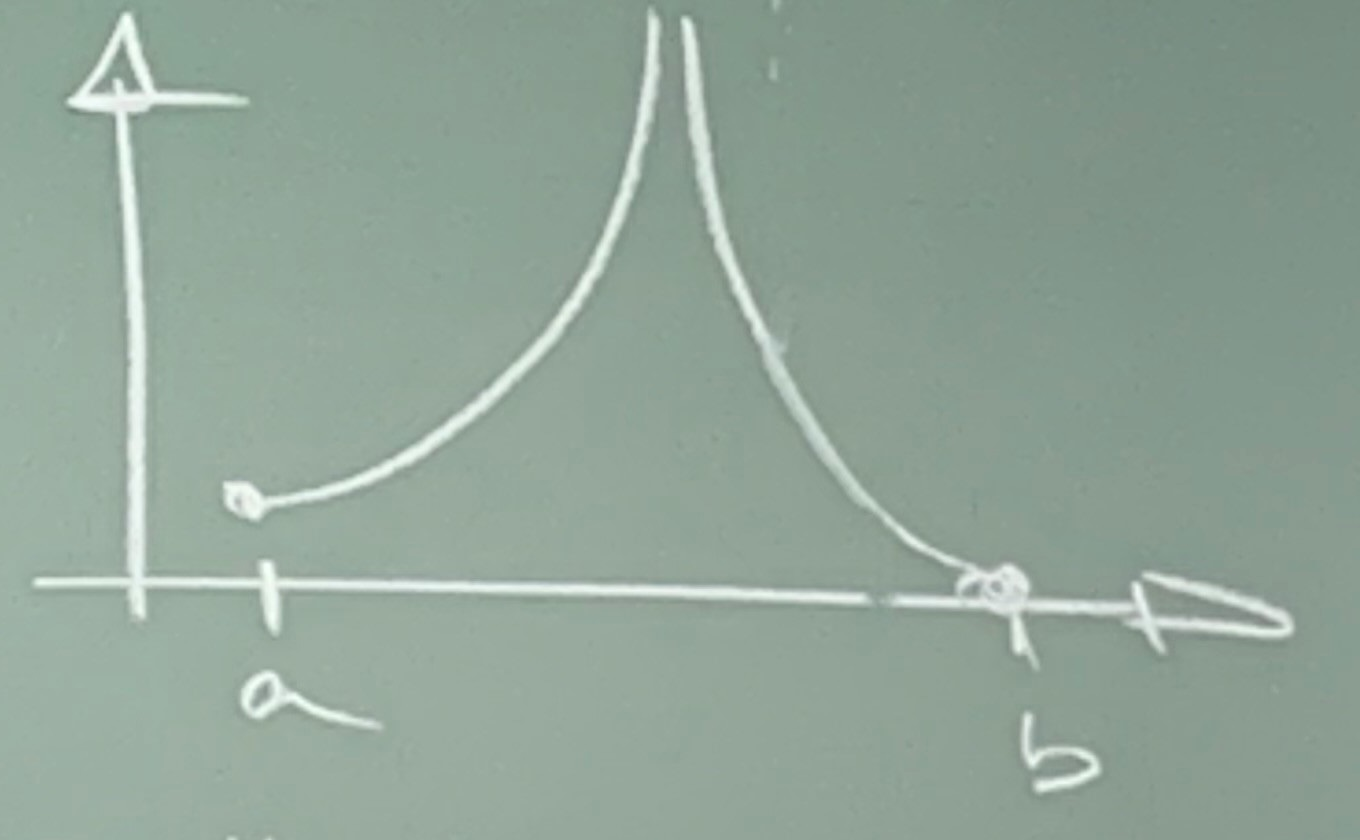
\includegraphics[scale=0.05]{lessons/lesson18/imgs/img03.jpg}% infoga bild 3 här
\end{itemize}
Integraler som involverar någon eller båda egenheterna ovan kallas för \\
\underline{generaliserade integraler}.
De definieras naturligt genom gränsvärden.
Om $f$ är obegränsad i en punkt $c\in[a,b]$ så definieras integralern $\int_a^b f(x)\, dx$ som:
\begin{equation*}
    \int_a^b f(x)\, dx =\lim_{z\to c^-}\int_a^z f(x)\, dx+ \lim_{z\to c^+}\int_z^b f(x)\, dx
\end{equation*}
Om några av integrationsgränserna är obegränsad definieras integralen $\in_{-\infty}^b f(x)\, dx$
och $\int_a^\infty f(x)\, dx$ som:
\begin{equation*}
    \int_{-\infty}^b f(x)\, dx=\lim_{R\to \infty}\int_R^b f(x)\, dx\text{ och }\int_a^\infty f(x)\, dx=\lim_{R\to \infty}\int_a^R f(x)\, dx
\end{equation*}
För generaliserade integraler kan en av tre olika fall inträffa:
\begin{enumerate}
    \item Integralen existerar (blir ett tal)
    \item Integralen existerar inte (gränsvärdet går inte att beräkna)
    \item Integralen $=\infty$ eller $-\infty$
\end{enumerate}
Om $1.$ så kallas integralen \underline{konvergent}.
För $2.$ så säger man att integralen är \underline{divergent} och för $3.$ divergent mot $\infty$ eller $-\infty$.
Går ibland att avgöra konvergens/divergent genom att jämföra generaliserade integraler mot varandra.
Om $-\infty\leq a<b \leq\infty$ och $f$ och $g$ är kontinuerliga på $(a,b)$ så att $0\leq f(x)\leq g(x)$ så konvergerar $\int_a^b f(x)\, dx$ om $\int_a^b g(x)\, dx$ gör det.
På samma sätt om $\int_a^b f(x)\, dx$ divergerar mot $\infty$ så gör också $\int_a^b g(x)\, dx$ det.

\paragraph{Ex (6.5.17)} Beräkna $\int_1^e\frac{dx}{x\sqrt{\ln(x)}}$
\subparagraph{Lösning}
Integralen är generaliserad eftersom $\ln(1)=0\Rightarrow\frac{1}{1\cdot\ln(1)}=\infty$.
Det gäller att
\begin{equation*}
    \frac{d}{dx}(\sqrt{ln(x)})=
    \frac{1}{2}\cdot(\ln(x))^{-\frac{1}{2}}\cdot\frac{1}{x}=
    \frac{1}{2}\frac{1}{x\sqrt{\ln(x)}}
\end{equation*}
\begin{equation*}
    \text{så }\int_1^e\frac{dx}{x\sqrt{\ln(x)}}=
    \lim_{z\to 1^+}\int_z^e\frac{dx}{x\sqrt{\ln(x)}}=
    \lim_{z\to 1^+}[2\sqrt{\ln(x)}]_z^e=
\end{equation*}
\begin{equation*}
    \lim_{z\to 1^+}2(\sqrt{\ln(e)}-\sqrt{\ln(z)})=
    2(1-0)=2\Rightarrow\text{Konvergent! }\Box
\end{equation*}

\paragraph{Ex (6.5.18)} Samma som innan för $\int_e^\infty\frac{dx}{x(\ln(x))^2}$
\subparagraph{Lösning}
\begin{equation*}
    \int_e^\infty\frac{dx}{x(\ln(x))^2}=
    \left\lbrace
    \begin{matrix}[c|c]
        u=\ln(x)            & x=e\Rightarrow u=1           \\
        du=\frac{1}{x}\, dx & x=\infty\Rightarrow u=\infty
    \end{matrix}
    \right.=
    \int_1^\infty\frac{1}{u^2}\, du=
\end{equation*}
\begin{equation*}
    \lim_{R\to\infty}\int_1^R\frac{1}{u^2}\, du=
    \lim_{R\to\infty}\int_1^R[-\frac{1}{u}]_1^R=
    \lim_{R\to\infty}((-\frac{1}{R})-(-\frac{1}{1}))=
    1\Rightarrow\text{Konvergent! }\Box
\end{equation*}
~\\
Några generaliserade integraler som är bra att känna till för att avgöra konvergens/divergens genom jämförelse är det så kallade "p-integralerna".
\begin{enumerate}
    \item $\int_a^\infty x^{-p}\, dx=
              \left\lbrace
              \begin{matrix}
                  \text{konvergerar mot }\frac{a^{1-p}}{p-1}\text{\underline{ om }} p>1 \\
                  \text{divergerar mot }\infty \text{ om } 0<p\leq 1
              \end{matrix}
              \right.$
    \item $\int_0^a x^{-p}\, dx=
              \left\lbrace
              \begin{matrix}
                  \text{konvergerar mot }\frac{a^{1-p}}{1-p}\text{\underline{ om }} 0<p<1 \\
                  \text{divergerar mot }\infty \text{ om } p\geq 1
              \end{matrix}
              \right.$
\end{enumerate}
för $0<a<\infty$.\\
%infoga bild 4
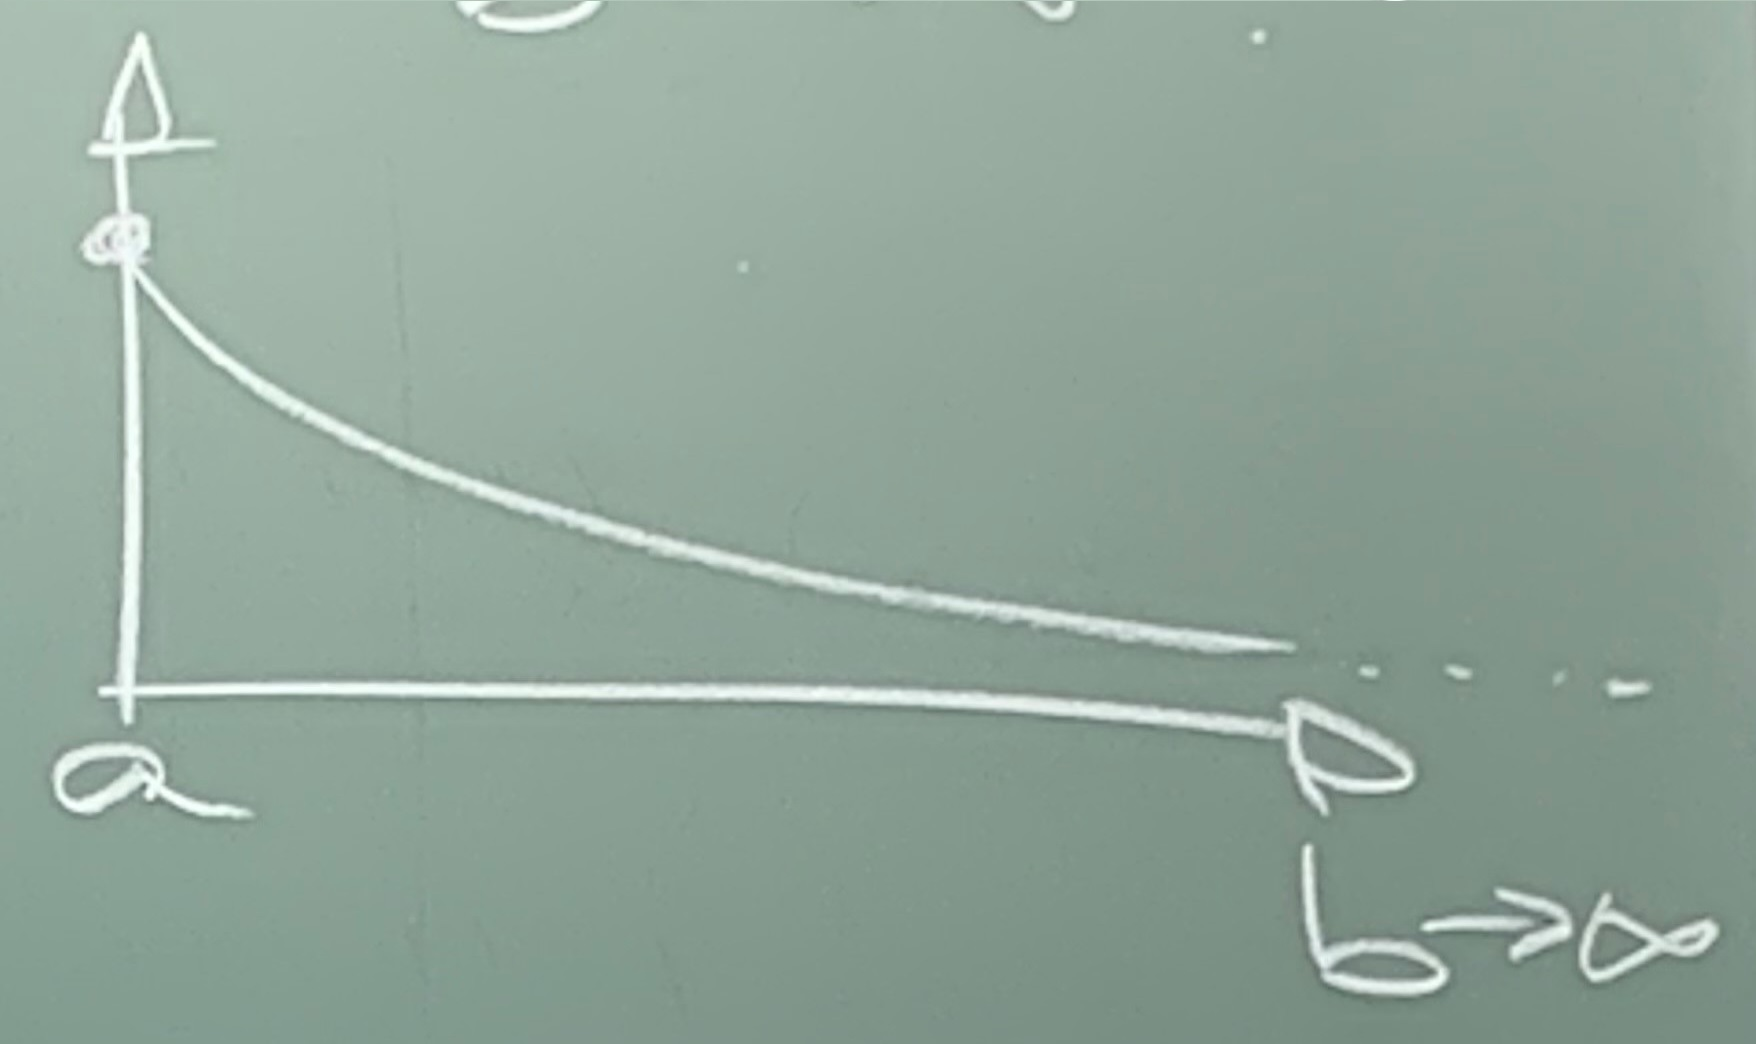
\includegraphics[scale=0.1]{lessons/lesson18/imgs/img04.jpg}

\chapter{Numerisk integration}
%Numerisk integration kommer inte på tentan 👀
Viktigt att kunna beräkna bra approximationer av integraler numeriskt.
Finns olika typer av algoritmer/metoder.

\section{Mittpunktsmetoden}
Approximera $\int_a^b f(x)\, dx$ som en Riemann-summa av staplar av samma bredd vars höjd motsvarar funktionens värde vid stapelns mittpunkt.\\
%infoga bild 5
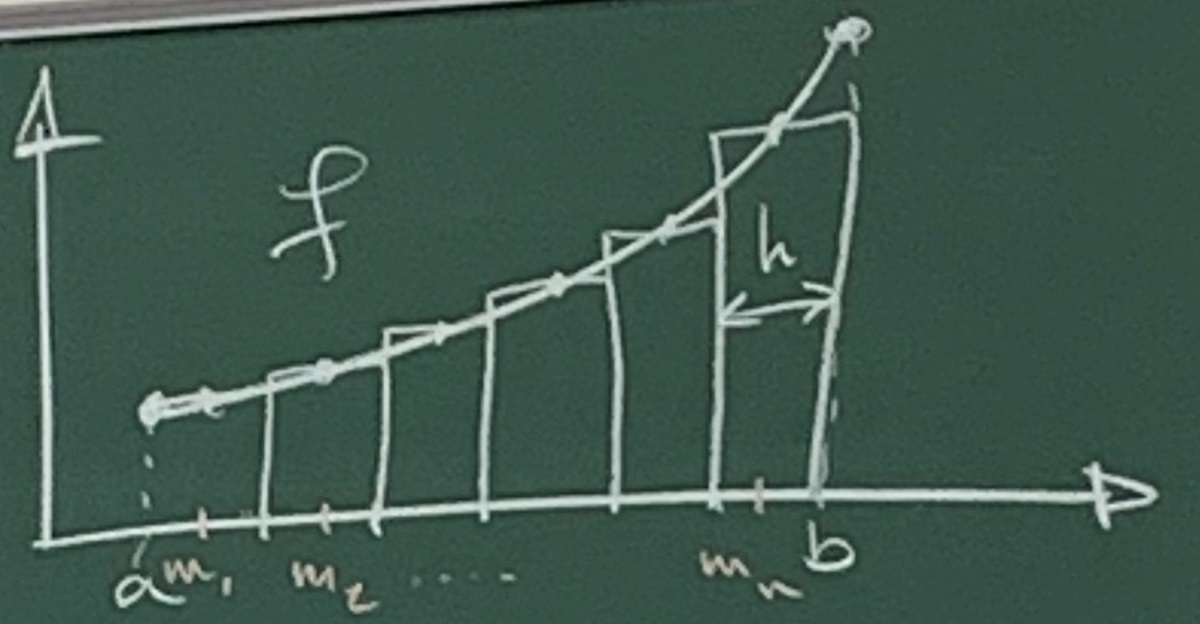
\includegraphics[scale=0.1]{lessons/lesson18/imgs/img05.jpg}
\begin{equation*}
    \Rightarrow \int_a^b f(x)\, dx \approx
    f(m_1)\cdot h+f(m_2)\cdot h+...+f(m_n)\cdot h=
    h\cdot\sum_i^n f(m_i)=
    M_n
\end{equation*}
Ju mindre bredd $h>0$ desto bättre approximation.

\section{Trapetsmetoden}
Istället för att som i mittpunktsmetoden använda en punkt per stapel för höjden (mittpunkten), används stapelsn ändpunkter och linjärapprox. funktionen.\\
%infoga bild 6
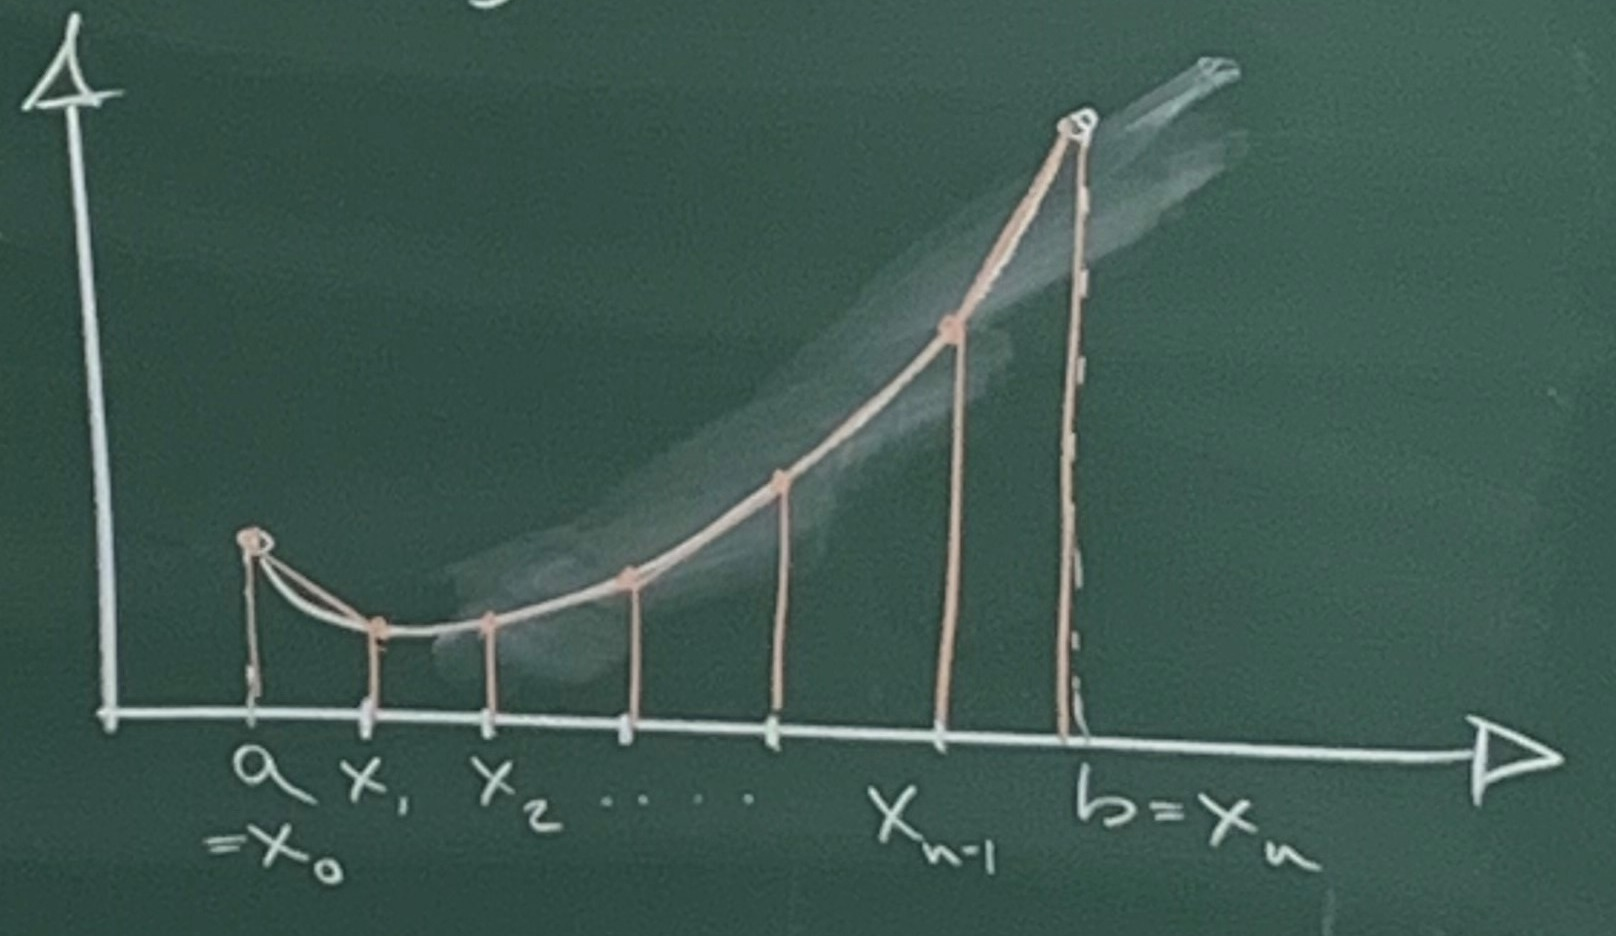
\includegraphics[scale=0.1]{lessons/lesson18/imgs/img06.jpg}\\
För stapel $i$ $(0<i<n)$ gäller:\\
%infoga bild 7
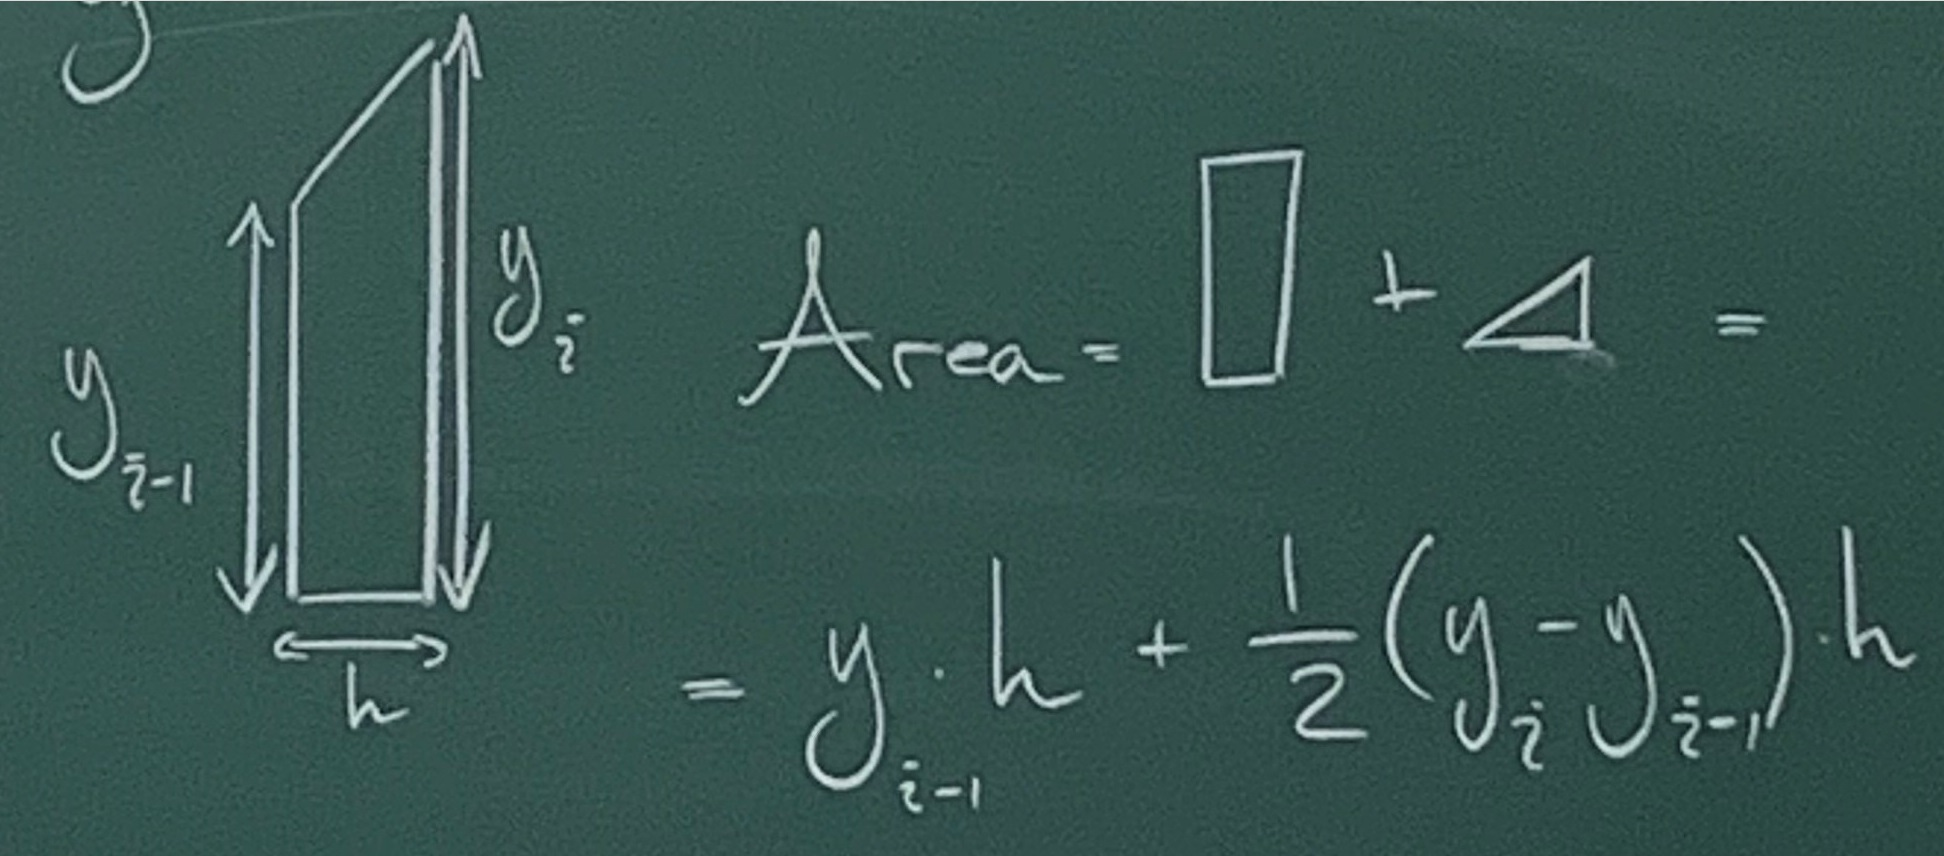
\includegraphics[scale=0.1]{lessons/lesson18/imgs/img07.jpg}
\begin{equation*}
    \Rightarrow \int_a^b f(x)\, dx\approx
    y_0\cdot h+\frac{1}{2}(y_1-y_0)\cdot h+y_1\cdot h+\frac{1}{2}(y_2-y_1)\cdot h+...=
\end{equation*}
\begin{equation*}
    h\cdot(\frac{1}{2}y_0+y_1+y_2+...+y_{n-1}+\frac{1}{2}y_n)=T_n
\end{equation*}
Vilken metod är bäst?
Man kan visa att:
\begin{itemize}
    \item Trapetsmetoden $|\int_a^b f(x)\, dx-M_n|\leq \frac{k\cdot(b-a)^3}{12n^2}$
    \item Mittpunktsmetoden $|\int_a^b f(x)\, dx-T_n\leq\frac{k\cdot(b-a)^3}{24n^2}$
\end{itemize}
för ett tal $K$ som hänger ihop med $f$.
Alltså är:
\begin{itemize}
    \item Trapetsmetoden $\int_a^b f(x)\, dx=M_n+O(\frac{1}{n^2})$
    \item Mittpunktsmetoden $\int_a^b f(x)\, dx=T_n+O(\frac{1}{n^2})$
\end{itemize}
dvs. dom är lika bra!\\
klar förbätttring fås genom att använda både mittpunkten och ändpunkterna och approximera $f$ i stapeln med en andragradskurva genom punkterna.
\section{Simpsons regel}
%infoga bild 8
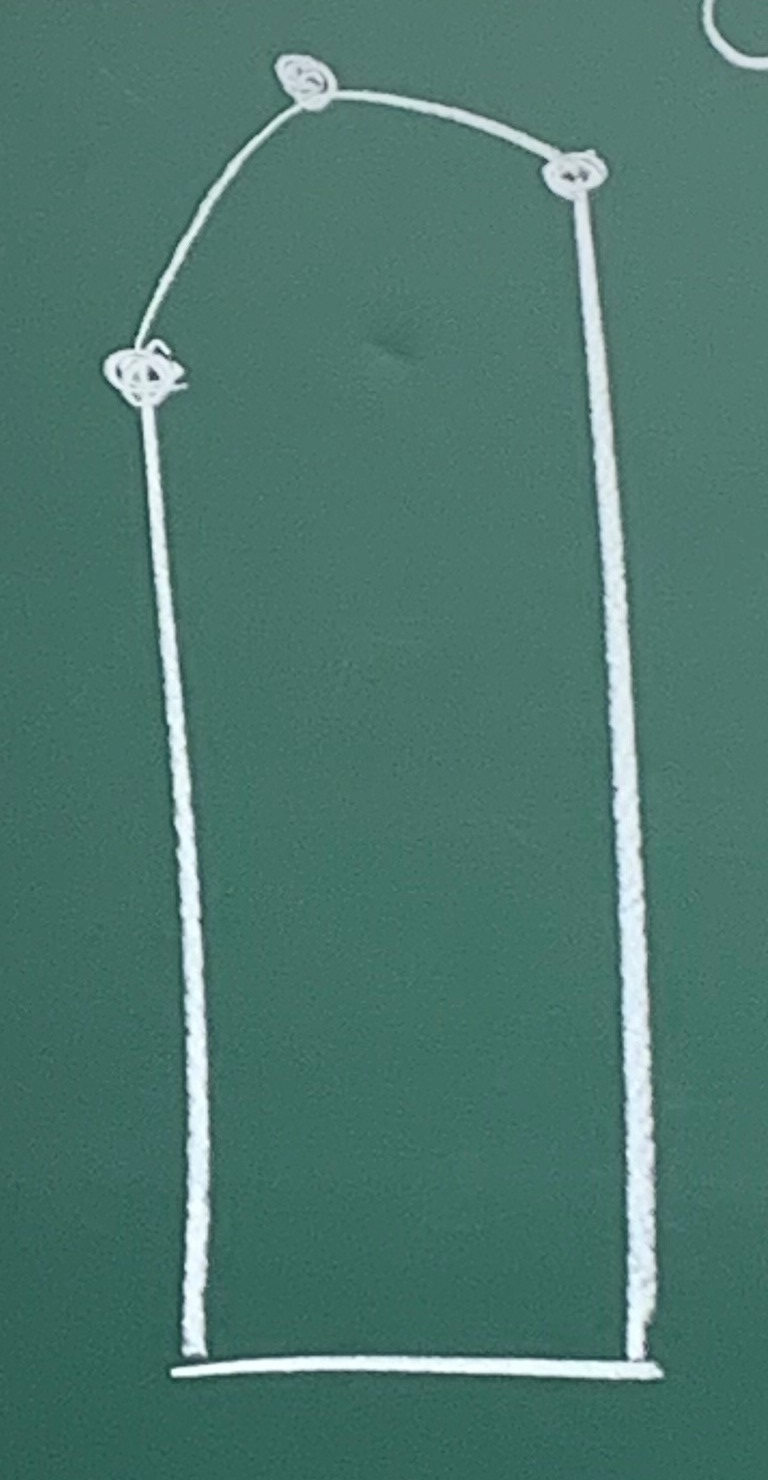
\includegraphics[scale=0.1]{lessons/lesson18/imgs/img08.jpg}\\
Man kan visa att Simpson-approximation innebär ett fel av storleksordning $O(\frac{1}{n^4})$ dvs.
\begin{equation*}
    \int_a^b f(x)\, dx=S_n+O(\frac{1}{n^4})
\end{equation*}